\chapter{Kalibrering}
\label{cha:kalibrering}

For at kunne oversætte mellem udstyrets kanalnummer og en given energi skulle der foretages en
kalibrering. Til dette formål blev der benyttet en kilde, der bestod af tre $\alpha$-kilder:
\ce{^{241}Am}, \ce{^{239}Pu} og \ce{^{244}Cm}.

Idet forstærkningen er indstillet forskelligt i de enkelte strips og sektorer, er det
nødvendigt at kalibrere dem enkeltvis. Linierne er skarpt adskilte, derfor kan kalibreringen udføres
ved at fitte lineært til deres centroid værdier.  

Det skulle dog vise sig ikke at være helt så nemt, idet detektoren havde et inativt område, der blot
bremsede partiklen uden at registre energien. Dette dødlag havde en tykkelse $\Delta x$ på et par
mikrometer. Dette er illustreret på \ref{fig:deadLayer}.

Dødlaget har den effekt, at partikler, der rammer længere ude på detektoren, vil miste mere energi
end de, der rammer de inderste strips, fordi de skal igennem en større vejlængde i dødlaget.

De relevante størrelser er den målte energi $E_{0}$, energien før dødlaget $E$ og vinklen $\phi$ mellem
partiklens hastighed og detektorens normal. Ud fra nogle enkelte geometriske betragtninger kan et
udtryk for $E$ opskrives
\begin{equation}
  \label{eq:deadE}
  E = E_{0} + \d{E}{x} \frac{\Delta x}{\cos \phi}  .
\end{equation}
Det sidste led er energitabet i dødlaget, som afhænger af stoppeevnen, $\d{E}{x}$, af
materialet. Denne antages konstant gennem dødlaget. 
\begin{figure}[h]
  \centering
  \includegraphics[width=7cm]{DeadLayer}
  \caption{Skematisk tegning af S3 dektoren med et dødlag.}
  \label{fig:deadLayer}
\end{figure}

\section{Estimation af dødlagets tykkelse}
\label{sec:dodlag}

For at kunne bestemme tykkelsen af dødlaget er det nødvendigt at kende energien ved forskellige
vinkler, men som sagt er forstærkningen indstillet forskelligt i ringene.

Løsningen på dette er at udvælge en radial sektor. Hver gang denne sektor bliver ramt, så findes den
med den tilsvarende cirkulære strip. Kriteriet for dette er, at kanalnumrerne stemmer overens inden
for en hvis usikkerhed. Dermed er det muligt at bestemme spektret for de enkelte cirkulære strips
udtrykt i kanalnummeret for den radiale sektor. Dermed er der ingen forstærkning at tage
højde for i spektrene.

I alle disse spektre bestemmes centroidværdien af \Pu toppen.
Centroidværdien blev normaliseret til kanalnummeret i strip 1 og blev plottet som funktion af
$1/{\cos \phi}$. Ud over dette er \cref{eq:deadE}, for forskellige tykkelser, også plottet. Disse er
normaliseret til det teoretiske udtryk for strip 1. Stoppeevnen er taget fra \cite{Ziegler}.

Det er ikke muligt at lave et fit til data med $\Delta x$ som en fri parameter, så derfor er tykkelsen af
dødlaget vurderet ud fra de teoretiske kurver, som er plottet på \cref{fig:dead}. Data er
konstistent med en tykkelse på hhv. \SI{3.3(5)}{\um} og \SI{4.2(5)}{\um} for op- og
nedstrømsdektektoren. En tilsvarende analyse er foretaget med S3 detektorerne roteret
180\degree. Her er var resultatet, at dødlaget var væsentlig mindre blot
\SI{0.6}{\um}. \fxfatal{Hvor præcis er disse tal?}

\begin{figure}[h]
  \centering
  \subbottom[Upstream]{\includegraphics[width=0.47\columnwidth]{DeadLayerThin}}%
  \hfill
  \subbottom[Downstream]{\includegraphics[width=0.47\columnwidth]{DeadLayerThick}}%
  \caption{De normaliserede energier som funktion af $1/{\cos\phi}$. Kurverne angiver det teoretiske
    udtryk givet i \cref{eq:deadE} og er plottet for forskellige tykkelser.}
  \label{fig:dead}
\end{figure}


\section{Kalibreringsalgoritmen}
\label{sec:kalalgo}

Når tykkelsen er kendt, kan den målte energi $E_{0}$ bestemmes. Dermed kan vores detektorer
kalibreres. Fordi energitabet både afhænger af indgangsenergien og hvilken partikel, der er tale om,
så er det nødvendigt, under databehandlingen, at bestemme energitabet for hver enkel hændelse.

For energier hvor stoppeevnen er stor, så vil det give anledning til en fejl, hvis energitabet anses
som konstant hele vejen igennem materialet. Det samlede tab skulle istedet udregnes som et
integral. Istedet benyttes middel rækkevidden af en partikel i et givent
materiale. Ækvivalent til \cref{eq:deadE} kan den samlede rækkevidde skrives som
\begin{equation}
  \label{eq:deadR}
  R(E) = R(E_{0}) + \frac{\Delta x}{\cos \phi} .
\end{equation}

Rækkeviden som funktion af energien er også tabuleret i \cite{Ziegler}, så for given hændelse blev
$R(E_{0})$ bestemt ved lineær interpolation mellem to de nærmeste tabulerede værdier. Til dette
adderet tykkelsen af dødlaget, hvor der blev taget højde for vinklen. Den samme tabel blev så
benyttet den modsatte vej, hvor energien blev bestemt ud fra den samlede rækkevidde. Der blev igen
benyttet lineær interpolation. 












